\section{Wykorzystane scenariusze}
Eksperymenty przeprowadzono na następujących scenariuszach, reprezentujących łatwy, sredni i wysoki poziom trudności.

\subsubsection{Podstawowy (ang. Basic)}\label{scenario_basic}
Sceneria składa się z prostokątnego pomieszczenia. Agent startuje w jednym końcu pomieszczenia, po środku ściany, a w losowym miejscu pod przeciwległą ścianą znajduje się pojedynczy, nieruchomy przeciwnik.

Agent może strzelać do przeciwnika oraz poruszać się w prawo lub w lewo. Agent ma ograniczoną amunicję i dostaje punkt za trafienie przeciwnika.

Strategia optymalna polega na przesunięciu się w kierunku przeciwnika i oddaniu do niego pojedynczego strzału.


\begin{figure}[H]
	\begin{floatrow}
		\ffigbox{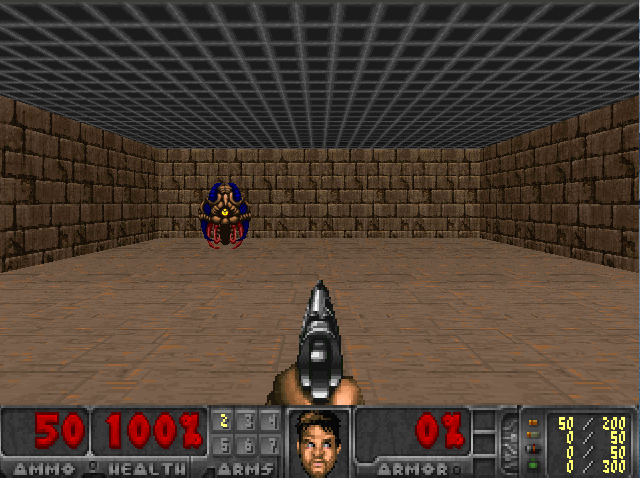
\includegraphics[scale = 0.35]{figures/screens/scenarios/basic.png}}{\caption{Scenariusz podstawowy}\label{fig:scenario_basic}}
	\end{floatrow}
\end{figure}

\subsubsection{Obrona środka (ang. Defend the center)}\label{scenario_dtc}
Sceneria składa się z kolistej areny. Agent znajduje się na środku areny, a na jej krańcach losowo pojawiają się przeciwnicy, którzy poruszają się w stronę agenta, a po dotarciu do niego zadają mu obrażenia. Są dwa rodzaje przeciwników różniących się wyglądem i szybkością poruszania.

Agent może strzelać i kręcić się wokół własnej osi w lewo i prawo. Agent ma ograniczoną amunicję i dostaje punkty za każde trafienie przeciwnika.

Strategia optymalna polega na kręceniu się w jedną strone w kółko, ignorowaniu odległych przeciwników i strzelaniu do bliskich, priorytetyzując szybszych przeciwników. Ignorowanie dalekich przeciwników jest konieczne, żeby w czasie strzelania do nich inni przeciwnicy nie zaszli agenta od tyłu - optymalna strategia wymaga zajmowania się najpierw najbliższym zagrożeniem.

\begin{figure}[H]
	\begin{floatrow}
		\ffigbox{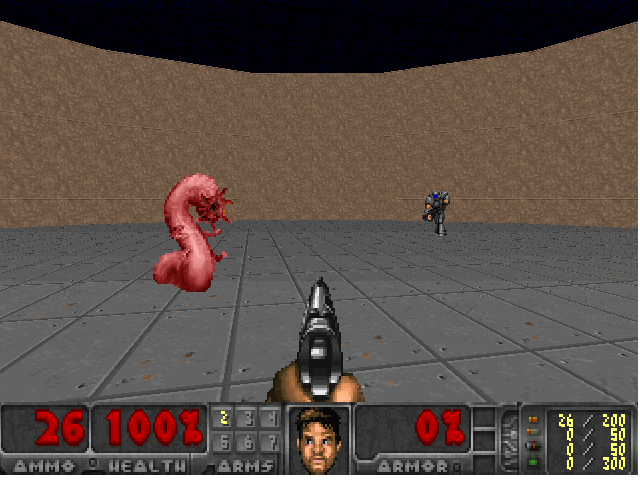
\includegraphics[scale = 0.35]{figures/screens/scenarios/dtc.png}}{\caption{Scenariusz obrona środka}\label{fig:scenario_dtc}}
	\end{floatrow}
\end{figure}


\subsubsection{Trudne zbieranie apteczek (ang. Health gathering supreme) }\label{scenario_hgs}
Sceneria składa się z labiryntu, którego podłoga jest pokryta kwasem. Agent startuje w losowym miejscu labiryntu. W tym scenariuszu nie ma ruchomych przeciwników. Na podłodze labiryntu pojawiają się losowo apteczki, które dodają agentowi punkty życia i miny, które zabierają agentowi punkty życia. Kwas na podłodze nieustannie odbiera agentowi punkty życia. 

Agent może poruszać się do przodu, na ukos w prawo lub w lewo oraz kręcić się wokół własnej osi w prawo lub w lewo. Agent dostaje punkty za pozostawanie przy życiu - im dłużej potrwa gra, tym większą sumę punktów zdobędzie agent.

Strategia optymalna polega na chodzeniu po labiryncie, niewchodzeniu na miny i zbieraniu apteczek, preferując kierowanie się do dużych skupisk apteczek. Wskazane jest unikanie zbierania pojedynczych, odizolowanych apteczek, gdyż liczba punktów życia uzyskana z takiej apteczki może być mniejsza niż liczba punktów życia straconych na dotarcie do apteczki. Wskazane jest niepozostawanie w jednym obszarze labiryntu, ponieważ nowe apteczki mogą nie pojawiać się wystarczająco szybko, żeby utrzymać agenta przy życiu.

Co istotne, w tym scenariuszu bardzo często optymalna decyzja nie jest jasna - sensownie działający ekspert i agent mogą często wybierać pomiędzy wieloma poprawnymi drogami i zachowaniami.

\begin{figure}[H]
	\begin{floatrow}
		\ffigbox{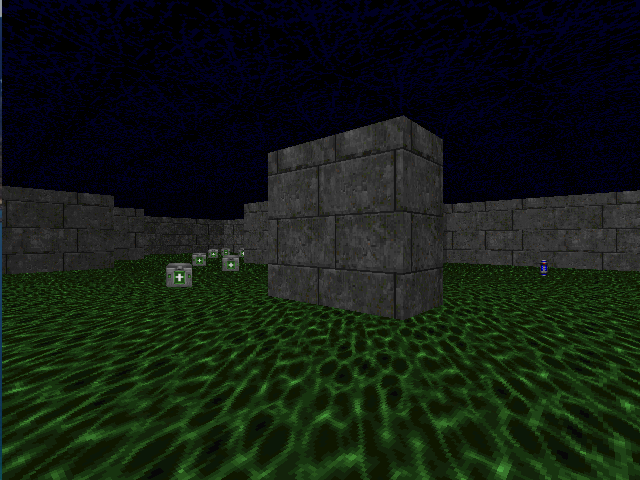
\includegraphics[scale = 0.35]{figures/screens/scenarios/hgs.png}}{\caption{scenariusz trudne zbieranie apteczek}\label{fig:scenario_hgs}}
	\end{floatrow}
\end{figure}
